% Options for packages loaded elsewhere
\PassOptionsToPackage{unicode}{hyperref}
\PassOptionsToPackage{hyphens}{url}
%
\documentclass[
]{article}
\title{Measuring Polarization in Online Communities\thanks{The code for this project is hosted on GitHub at \href{https://github.com/wlgfour/social_networks}{wlgfour/social\_networks}}}
\usepackage{etoolbox}
\makeatletter
\providecommand{\subtitle}[1]{% add subtitle to \maketitle
  \apptocmd{\@title}{\par {\large #1 \par}}{}{}
}
\makeatother
\subtitle{using exponential family random graph models and sentiment analysis}
\author{William Gerecke}
\date{28 April 2022}

\usepackage{amsmath,amssymb}
\usepackage{lmodern}
\usepackage{iftex}
\ifPDFTeX
  \usepackage[T1]{fontenc}
  \usepackage[utf8]{inputenc}
  \usepackage{textcomp} % provide euro and other symbols
\else % if luatex or xetex
  \usepackage{unicode-math}
  \defaultfontfeatures{Scale=MatchLowercase}
  \defaultfontfeatures[\rmfamily]{Ligatures=TeX,Scale=1}
\fi
% Use upquote if available, for straight quotes in verbatim environments
\IfFileExists{upquote.sty}{\usepackage{upquote}}{}
\IfFileExists{microtype.sty}{% use microtype if available
  \usepackage[]{microtype}
  \UseMicrotypeSet[protrusion]{basicmath} % disable protrusion for tt fonts
}{}
\makeatletter
\@ifundefined{KOMAClassName}{% if non-KOMA class
  \IfFileExists{parskip.sty}{%
    \usepackage{parskip}
  }{% else
    \setlength{\parindent}{0pt}
    \setlength{\parskip}{6pt plus 2pt minus 1pt}}
}{% if KOMA class
  \KOMAoptions{parskip=half}}
\makeatother
\usepackage{xcolor}
\IfFileExists{xurl.sty}{\usepackage{xurl}}{} % add URL line breaks if available
\IfFileExists{bookmark.sty}{\usepackage{bookmark}}{\usepackage{hyperref}}
\hypersetup{
  pdftitle={Measuring Polarization in Online Communities},
  pdfauthor={William Gerecke},
  pdfkeywords={Social networks, Exponential family Random Graph Model, ERGM, Polarization, Sentiment analysis},
  hidelinks,
  pdfcreator={LaTeX via pandoc}}
\urlstyle{same} % disable monospaced font for URLs
\usepackage[margin=1in]{geometry}
\usepackage{longtable,booktabs,array}
\usepackage{calc} % for calculating minipage widths
% Correct order of tables after \paragraph or \subparagraph
\usepackage{etoolbox}
\makeatletter
\patchcmd\longtable{\par}{\if@noskipsec\mbox{}\fi\par}{}{}
\makeatother
% Allow footnotes in longtable head/foot
\IfFileExists{footnotehyper.sty}{\usepackage{footnotehyper}}{\usepackage{footnote}}
\makesavenoteenv{longtable}
\usepackage{graphicx}
\makeatletter
\def\maxwidth{\ifdim\Gin@nat@width>\linewidth\linewidth\else\Gin@nat@width\fi}
\def\maxheight{\ifdim\Gin@nat@height>\textheight\textheight\else\Gin@nat@height\fi}
\makeatother
% Scale images if necessary, so that they will not overflow the page
% margins by default, and it is still possible to overwrite the defaults
% using explicit options in \includegraphics[width, height, ...]{}
\setkeys{Gin}{width=\maxwidth,height=\maxheight,keepaspectratio}
% Set default figure placement to htbp
\makeatletter
\def\fps@figure{htbp}
\makeatother
\setlength{\emergencystretch}{3em} % prevent overfull lines
\providecommand{\tightlist}{%
  \setlength{\itemsep}{0pt}\setlength{\parskip}{0pt}}
\setcounter{secnumdepth}{5}
\newlength{\cslhangindent}
\setlength{\cslhangindent}{1.5em}
\newlength{\csllabelwidth}
\setlength{\csllabelwidth}{3em}
\newlength{\cslentryspacingunit} % times entry-spacing
\setlength{\cslentryspacingunit}{\parskip}
\newenvironment{CSLReferences}[2] % #1 hanging-ident, #2 entry spacing
 {% don't indent paragraphs
  \setlength{\parindent}{0pt}
  % turn on hanging indent if param 1 is 1
  \ifodd #1
  \let\oldpar\par
  \def\par{\hangindent=\cslhangindent\oldpar}
  \fi
  % set entry spacing
  \setlength{\parskip}{#2\cslentryspacingunit}
 }%
 {}
\usepackage{calc}
\newcommand{\CSLBlock}[1]{#1\hfill\break}
\newcommand{\CSLLeftMargin}[1]{\parbox[t]{\csllabelwidth}{#1}}
\newcommand{\CSLRightInline}[1]{\parbox[t]{\linewidth - \csllabelwidth}{#1}\break}
\newcommand{\CSLIndent}[1]{\hspace{\cslhangindent}#1}
\usepackage{booktabs}
\usepackage{longtable}
\usepackage{array}
\usepackage{multirow}
\usepackage{wrapfig}
\usepackage{float}
\usepackage{colortbl}
\usepackage{pdflscape}
\usepackage{tabu}
\usepackage{threeparttable}
\usepackage{threeparttablex}
\usepackage[normalem]{ulem}
\usepackage{makecell}
\usepackage{xcolor}
\ifLuaTeX
  \usepackage{selnolig}  % disable illegal ligatures
\fi

\begin{document}
\maketitle
\begin{abstract}
With the growth of the internet and social media platforms, it is increasingly easy for communities of like-minded people to form. This can be good, but often results in people strengthening beliefs by affirmation rather than by a decision making process. In this paper, I use Exponential Random Graph Models and sentiment analysis to measure polarization in online communities, specifically on the site Reddit. \textbf{I find that ???}. As such, it is important for companies that make social media sites as well as individuals using the sites to consider the impact of forming homogeneous communities in the future.

\par

\textbf {Keywords:} Social networks, Exponential family Random Graph Model, ERGM, Polarization, Sentiment analysis
\end{abstract}

\newpage
\tableofcontents

\newpage

\hypertarget{introduction}{%
\section{Introduction}\label{introduction}}

With the popularization of the internet, and increasing ease of access, social media is becoming ubiquitous in modern society. These platforms facilitate instant communication between individuals, or between an individual and large audience. Beyond the ease and availability of such communication, social media platforms are run by highly-engineered algorithms that are designed to find people and communities that are similar to each other. For people like hobbyists, this is good since it allows people from niche groups to find each other easily. It is possible, however, to see that this could have a polarizing effect in a different scenario. For example, people with political beliefs are presented with like-minded opinions from around the world, and such communities strengthen their beliefs by affirmation, rather than by a decision making process. As such, it is important to be able to measure and understand the effect that online communities have on the people that participate in them, and the behaviors exhibited therein

Many social media platforms can be represented as graphs, as they represent an underlying social network of individuals. Graphs are data structures that are represented by a set of nodes \(V\) and a set of edges \(E\subseteq\{(x,y)\in V^2,x\not=y\}\) which represent a connection between nodes. There are countless phenomena that can be represented by this data structure, such as roads, mathematical operations, supply chains, the internet, social networks, and more. As such, understanding and modelling graphical structures is crucial to understanding the universe that we live in, and has been a topic of much research. The problem with graphical structures is that typical assumptions of independence are violated by many of the scenarios that are represented by graphs. For example, in a social network where people share an edge if they are friends, the probability of sharing an edge is no longer independent. This is because it is reasonable that sharing a mutual friend will influence the probability of a friendship. Statisticians have developed Exponential family Random Graph Models (ERGMs) in order to allow for the representation of these dependent relationships.

In this paper, I look at polarization in online communities, specifically on the social media platform Reddit. For the purpose of this paper, I define polarization as the tendency for people to respond positively in the presence of positive sentiments, and negatively in the presence of negative sentiments. That is, polarization is defined to be when individuals in a community have views and opinions that align. I use a graph to represent interactions within communities on the Reddit, and sentiment analysis to classify individual interactions as positive or negative. \textbf{I find that ????}.

I begin by describing how the data is gathered, cleaned, and parsed into a graphical structure. I proceed to elaborate on the model used for sentiment analysis, and the structure of ERGMs. After that, I discuss the results of applying these models to the data that was gathered in order to measure polarization in online communities. Finally I discuss the impact of the results, weaknesses with the approach presented, and suggest directions for future research.

\hypertarget{data}{%
\section{Data}\label{data}}

\hypertarget{software}{%
\subsection{Software}\label{software}}

The R programming language (R Core Team 2021) was used to generate the report, data, and analyses associated with this project. The \texttt{purrr}, \texttt{dplyr}, \texttt{stringr}, and \texttt{tidyr} were used for data manipulation Wickham (2021). Data was simulated using the \texttt{stringi} and \texttt{keyToEnglish} packages Candocia (2021). The \texttt{vader}, which exposed an R API for the Vader NLP model was used to generate sentiment labels for the data (Hutto and Gilbert 2014). \texttt{jsonlite} was used to scrape data from Reddit using Reddit's json API (Ooms 2014). The \texttt{statnet} package was used to generate network data structures, as well as fit ERGM models Hunter et al. (2008). Finally, the code and data are hosted on GitHub ({``Where the World Builds Software,''} n.d.).

\hypertarget{reddit}{%
\subsection{Reddit}\label{reddit}}

The site Reddit was used to gather data for this project. Reddit is structured such that there are communities that users can subscribe to called subreddits. When someone creates a post, the post is categorized under a subreddit. Once a post is created, users can then comment on a post, as well as other comments. ``Has-a'' relationships are as follows:

\begin{itemize}
\tightlist
\item
  subreddit: N/A
\item
  post: subreddit, author
\item
  comment: parent (post or comment), subreddit, author
\end{itemize}

That is, a post has a subreddit and author that it is associated with. This project uses a dataset composed of instances of comments which have a parent, author, and subreddit associated with them, in addition to a comment body (text), and other metadata.

\hypertarget{gathering}{%
\subsection{Gathering}\label{gathering}}

Data was gathered using the Reddit json API. Given any Reddit url \texttt{u}, a json string representing that url can be obtained by downloading the url given by \texttt{\{url\}/.json}. The algorithm for scraping comments is as follows:

\begin{enumerate}
\def\labelenumi{\arabic{enumi}.}
\tightlist
\item
  Initialize \texttt{links} to have top posts from some seed communities. Initialize \texttt{comments} to be empty
\item
  Randomly select a \texttt{link} from \texttt{links}
\item
  Append all comments from \texttt{link} to \texttt{comments}
\item
  If \texttt{link} represents a use: add the posts from the users most recent comments to \texttt{links}
\item
  If \texttt{link} represents a post: add the users from the posts comments to \texttt{links}
\item
  Remove duplicates in \texttt{comments} and \texttt{links}. Remove \texttt{links} that have already been visited. Remove rows in \texttt{comments} that contain \texttt{NA} values.
\item
  Goto 2.
\end{enumerate}

At the start of the algorithm, a cache file is generated, and the algorithm caches \texttt{comments} every 10 iterations. For this project, the seed was set to three of the most active subreddits, `AskReddit,' `worldnews,' and `gifs' (reddit 2011).

\begin{table}

\caption{\label{tab:rawdata}The table shows the summary statistics for the 15 subredits with the most comments recorded, and the total summary statistics for all subreddits visited.}
\centering
\begin{tabular}[t]{lrrr}
\toprule
Subreddit & Posts & Unique users & Average replies per comment\\
\midrule
AskReddit & 22,605 & 3,829 & 1.66\\
worldnews & 13,992 & 2,795 & 1.45\\
gifs & 1,521 & 1,125 & 2.76\\
ukraine & 1,492 & 327 & 1.15\\
news & 1,163 & 555 & 1.17\\
\addlinespace
politics & 1,051 & 366 & 1.20\\
AmItheAsshole & 875 & 207 & 1.18\\
funny & 790 & 473 & 1.27\\
interestingasfuck & 788 & 449 & 1.15\\
technology & 763 & 369 & 1.19\\
\addlinespace
movies & 694 & 360 & 1.16\\
Damnthatsinteresting & 644 & 311 & 1.16\\
AskMen & 632 & 204 & 1.25\\
antiwork & 628 & 310 & 1.26\\
mildlyinteresting & 539 & 338 & 1.17\\
\midrule
\addlinespace
Total & 117,437 & 44,108 & 1.02\\
\bottomrule
\end{tabular}
\end{table}

Statistics for the raw data that was gathered can be seen in table \ref{tab:rawdata}. There were 7208 subreddits visited, but the data collected for most of them was fairly sparse. It is important to note that when Reddit returns information, it hides many of the comments in a post by default. It is possible to retrieve the hidden comments by expanding certain links, but I did not do that for this project, which explains why the comment multiplicity is so low, averaging between 1 and 2 in the dataset. We can also see that significantly more comments have been gathered from AskReddit than any other subreddit. This is probably because this was one of the seed communities, and the posts on AskReddit ahve a high multiplicity. As such, many links were gathered from AskReddit early, making it more likely to gather more links from AskReddit, which in turn makes it more likely to gather even more links from AskReddit. This is an artifact of the algorithm that I used to scrape data, and the report would benifit from designing an algorithm that does not have this weakness.

\hypertarget{cleaning}{%
\subsection{Cleaning}\label{cleaning}}

Once the data scraping script is run, and there are one or more chunks of raw data, the data are combined, filtered, and labelled with sentiment scores. Due to computational constraints, the amount of data that was processed had to be severely limited. The first computational constraint came from generating sentiment scores, which is a very computationally intensive process. The second is fitting the model, and assessing its goodness of fit, which was another source of significant computational burden. Even with ample time, R experienced frequent crashes, indicating that in order to perform analyses on the entire dataset or a larger sample, better software design is important.

The filtering process excluded portions of the data for two reasons. One is because there weren't enough data points, and the second is because there were too many data points for the analyses to be computationally feasible. Data were first gathered and grouped by subreddit. Then data from a subreddit with fewer than 500 recorded comments were dropped. Finally, if a subreddit had more than 1000 recorded comments, 1000 were selected at random.

The sentiment scoring process was the main computational bottleneck in the data preparation process. With better software design, the process cold be parallelized to greatly speed up the labeling process and allow for larger datasets. This, however, would likely need to be done outside of the R language because even when run using only one thread on about 20,000 comments, the R garbage collection process caused the program to crash repeatedly.

\hypertarget{graph-construction}{%
\subsection{Graph construction}\label{graph-construction}}

In order to create the graphical representation of the data, it was important to develop a scheme that represented the underlying structure of interactions that are present in the online conversations gathered. Several different approaches were considered, and the one that was selected is outlined below. It is important to note that there is likely a better design that allows for better representations of the data. It is also important to note that the way the graph is constructed directly influences how accurately it represents the network as well as the computational feasibility of the models that operate over the graphical representations.

\begin{figure}

{\centering 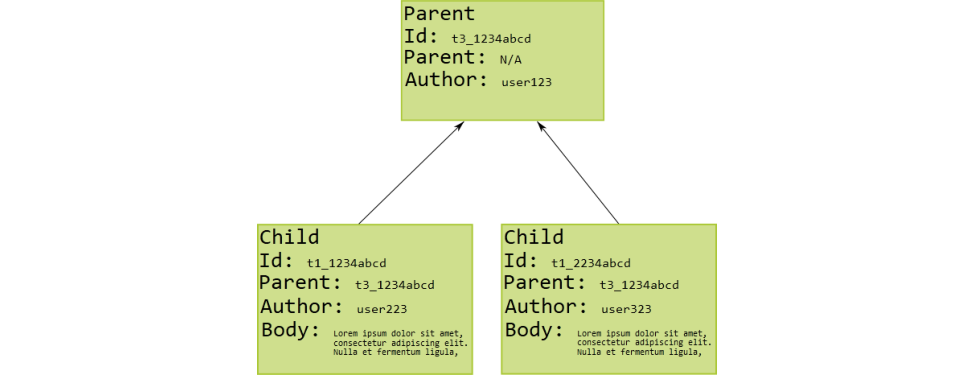
\includegraphics{E:/School/STA304/social_networks/outputs/report/report_files/figure-latex/graph-1} 

}

\caption{The figure shows the relationships expressed by the graphical construction used by this project. Each square represents a node, and the text contained within represents the attributes associated with each node. The parent in this case represents a post, and would not have a body, but it could also be a comment.}\label{fig:graph}
\end{figure}

Figure \ref{fig:graph} describes the graphical structure that is used in this project. Consider the data examined by this project to be a social network. Social networks can be represented as a graph with nodes \(V\) and edges \(E\subseteq V\times V\). I decided to use a directed graph where each node represents a post or comment. Nodes have an associated sentiment, author, subreddit, parent, and ID as seen below:

\begin{verbatim}
    node <- {
      .sentiment
      .author
      .subreddit
      .parent
      .id
    }
\end{verbatim}

There are two constraints on the nodes:

\begin{enumerate}
\def\labelenumi{\arabic{enumi}.}
\tightlist
\item
  \(node.sentiment\in[-1,1]\)
\item
  \(\{node.parent|node\in V\}\equiv \{node.id|node\in V\}\)
\end{enumerate}

Exceptions to these rules are posts themselves, since top level comments are all direct children of posts, which do not have a parent or sentiment. In this case, \(parent.parent=NA\), and is not included in the graph. The result of this is that comment chains will appear as inverted trees.

Since the graph is directional, the existence of an edge \((u,v)\in E\) does not guarantee the existence of edge \((v,u)\). In fact, because comments on Reddit form a tree, and each comment can only be a reply to one parent, this explicitly guarantees that \((v,u)\not\in E\). Another side effect of the fact that each node will only originate one edge is that the graph will be very sparse, with \(|E|\in\mathcal{O}(V)\).

Furthermore, I define one graph for each subreddit, \(sub\), as the graph over the nodes \(V_{sub}\equiv\{n|n.subreddit=sub,\ n\in V\}\). Note that there are no edges that need to be severed due to this construction because any comment will explicitly be a reply to some media that was posted in that subreddit. Thus, \(G_{sub}=(V_{sub},E_{sub})\) is a straightforward construction.

\hypertarget{model}{%
\section{Model}\label{model}}

\hypertarget{sentiment-analysis}{%
\subsection{Sentiment Analysis}\label{sentiment-analysis}}

Sentiment analysis was done using the Vader (Valance Aware Dictionary for sEntiment Reasoning) model from NLP that was specifically designed to perform well on content from the internet (Hutto and Gilbert 2014). VADER is capable of identifying polarity and intensity of the sentiment expressed by text and returns a composite sentiment score between -1 and 1, where -1 represents a strong negative sentiment, 0 is neutral, and 1 represents a strong positive sentiment.

VADER uses a dictionary to identify lexical fragments and assign sentiment scores (intensity and polarity) to components of the body of text. The dictionary that maps lexical features to sentiment scores was trained using manually labeled data. VADER is also capable of understanding contextualization such as ``I don't like this,'' as well as non-standard contractions such as ``like'nt'' by using some simple heuristics that the authors decided on. The scores assigned to lexical components are then averaged, and normalized.

\hypertarget{ergm}{%
\subsection{ERGM}\label{ergm}}

The model used to understand the graphical structure of the data which is examined in this report is the ERGM. This is because typical statistical models assume that the observations that they operate over are independent of each other. For example, if two people are friends on a social network, they are more likely to interact with each others' media, hence increasing the probability of an edge between them, and invalidating the assumption that they are independent of each other. In order to account for the dependence between the observations, we need to use a model that takes into account the underlying representation of the dataset. The ERGM is analogous to the generalized linear model, but takes into account the underlying structure of the graph, which is why it's appropriate for this application.

Given an observed network, the ERGM estimates the parameters of an expontential family model that takes the form of a log-linear combination of feature weights (Wyatt, Choudhury, and Bilmes 2009): \[
p(\mathbf{Y}=y)=\frac{1}{Z_\eta}{e^\eta}^\top\phi(y)
\]

Where:

\begin{itemize}
\tightlist
\item
  \(\mathbf{Y}\) are weights representing the edges of the graph
\item
  \(\phi\) defines the features over \(y\)
\item
  \(\eta\) is a vector of weights
\item
  \(Z_\eta\) is a normalizing constant
\end{itemize}

Typically, features account for the structural dependencies int he graph, allowing the model to more intuitively reason over the graphical structure of the data. The problem with using these models in practice, though, is that models are highly prone to degeneracy. In order to assess model degeneracy, it is important to examine the goodness of fit (GOF) which uses the generative nature of the estimated ERGM to find simulated networks. The simulated networks are then used to provide estimates for features such as node degree, edgewise shared partners, and geodesic distance. If the estimated networks align with the observed network, the model can be said to be robust.

\hypertarget{results}{%
\section{Results}\label{results}}

\hypertarget{discussion}{%
\section{Discussion}\label{discussion}}

\hypertarget{findings}{%
\subsection{Findings}\label{findings}}

\hypertarget{weaknesses}{%
\subsection{Weaknesses}\label{weaknesses}}

\begin{itemize}
\tightlist
\item
  scraping algotithm visits some subreddits more often
\item
  scraping didn't expand hidden comments
\item
  computational tractability

  \begin{itemize}
  \tightlist
  \item
    small dataset
  \end{itemize}
\end{itemize}

\hypertarget{future-work}{%
\subsection{Future work}\label{future-work}}

\newpage

\hypertarget{references}{%
\section{References}\label{references}}

\hypertarget{refs}{}
\begin{CSLReferences}{1}{0}
\leavevmode\vadjust pre{\hypertarget{ref-keyToEnglish}{}}%
Candocia, Max. 2021. \emph{keyToEnglish: Convert Data to Memorable Phrases}. \url{https://CRAN.R-project.org/package=keyToEnglish}.

\leavevmode\vadjust pre{\hypertarget{ref-stringi}{}}%
Gagolewski, Marek. 2021. \emph{Stringi: Fast and Portable Character String Processing in r}. \url{https://stringi.gagolewski.com/}.

\leavevmode\vadjust pre{\hypertarget{ref-statnet}{}}%
Handcock, Mark S., David R. Hunter, Carter T. Butts, Steven M. Goodreau, Pavel N. Krivitsky, and Martina Morris. 2018. \emph{Ergm: Fit, Simulate and Diagnose Exponential-Family Models for Networks}. The Statnet Project (\url{http://www.statnet.org}). \url{https://CRAN.R-project.org/package=ergm}.

\leavevmode\vadjust pre{\hypertarget{ref-purrr}{}}%
Henry, Lionel, and Hadley Wickham. 2020. \emph{Purrr: Functional Programming Tools}. \url{https://CRAN.R-project.org/package=purrr}.

\leavevmode\vadjust pre{\hypertarget{ref-ergm}{}}%
Hunter, David R., Mark S. Handcock, Carter T. Butts, Steven M. Goodreau, and Martina Morris. 2008. {``Ergm: A Package to Fit, Simulate and Diagnose Exponential-Family Models for Networks.''} \emph{Journal of Statistical Software} 24 (3): 1--29.

\leavevmode\vadjust pre{\hypertarget{ref-vader}{}}%
Hutto, Clayton, and Eric Gilbert. 2014. {``Vader: A Parsimonious Rule-Based Model for Sentiment Analysis of Social Media Text.''} In \emph{Proceedings of the International AAAI Conference on Web and Social Media}, 8:216--25. 1.

\leavevmode\vadjust pre{\hypertarget{ref-jsonlite}{}}%
Ooms, Jeroen. 2014. {``The Jsonlite Package: A Practical and Consistent Mapping Between JSON Data and r Objects.''} \emph{arXiv:1403.2805 {[}Stat.CO{]}}. \url{https://arxiv.org/abs/1403.2805}.

\leavevmode\vadjust pre{\hypertarget{ref-r}{}}%
R Core Team. 2021. \emph{R: A Language and Environment for Statistical Computing}. Vienna, Austria: R Foundation for Statistical Computing. \url{https://www.R-project.org/}.

\leavevmode\vadjust pre{\hypertarget{ref-reddit}{}}%
reddit. 2011. {``Reddit.''} \url{http://reddit.com}.

\leavevmode\vadjust pre{\hypertarget{ref-git}{}}%
{``Where the World Builds Software.''} n.d. \emph{GitHub}. \url{https://github.com/}.

\leavevmode\vadjust pre{\hypertarget{ref-stringr}{}}%
Wickham, Hadley. 2019. \emph{Stringr: Simple, Consistent Wrappers for Common String Operations}. \url{https://CRAN.R-project.org/package=stringr}.

\leavevmode\vadjust pre{\hypertarget{ref-tidyr}{}}%
---------. 2021. \emph{Tidyr: Tidy Messy Data}. \url{https://CRAN.R-project.org/package=tidyr}.

\leavevmode\vadjust pre{\hypertarget{ref-dplyr}{}}%
Wickham, Hadley, Romain François, Lionel Henry, and Kirill Müller. 2021. \emph{Dplyr: A Grammar of Data Manipulation}. \url{https://CRAN.R-project.org/package=dplyr}.

\leavevmode\vadjust pre{\hypertarget{ref-wyatt}{}}%
Wyatt, Danny, Tanzeem Choudhury, and Jeff Bilmes. 2009. {``Dynamic Multi-Valued Network Models for Predicting Face-to-Face Conversations.''} In \emph{NIPS Workshop on Analyzing Networks and Learning with Graphs}. Citeseer.

\end{CSLReferences}

\end{document}
